% ID: SEL-D0018-BB-E04
% ESTADO: validada. S019. Revisión matemática, didáctica y visual.
\textbf{a) Continuidad y derivabilidad.}\par\nopagebreak[4]
El dominio es $\mathbb R$ porque el denominador $x+1$ se usa sólo para $x<-2$. En el empalme, el límite izquierdo vale $-2$ y $f(-2)=4+a$. La continuidad exige $\boxed{a=-6}$. Para ese valor, las pendientes laterales son
\[
-\frac{2}{(-2+1)^2}=-2,\qquad 2(-2)=-4.
\]
La función es derivable en el interior de cada tramo y presenta una esquina en $x=-2$.

\textbf{b) Tangente en $x=3$.}\par\nopagebreak[4]
En el tramo cuadrático, $f(3)=3$ y $f'(3)=6$. Resulta $\boxed{y=6x-15}$.

\textbf{c) Esbozo y área.}\par\nopagebreak[4]
El tramo racional desciende desde valores próximos a $0$ por debajo del eje hasta el empalme $(-2,-2)$. El tramo cuadrático desciende hasta $(0,-6)$ y luego crece. Su única raíz dentro de ese tramo es $\sqrt6$. En $[3,5]$ la gráfica queda por encima del eje.
\begin{center}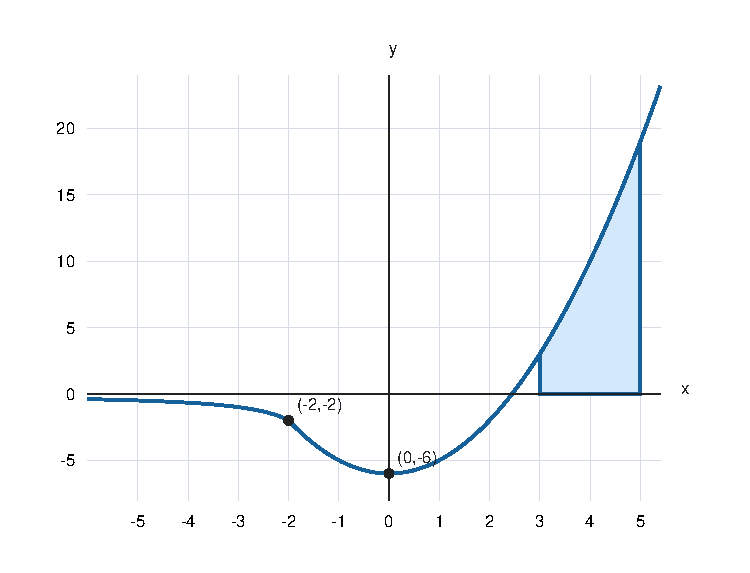
\includegraphics[width=0.55\linewidth]{recursos/figuras/s019-area.pdf}\end{center}
\[
\mathcal A=\int_3^5(x^2-6)\,dx
=\left[\frac{x^3}{3}-6x\right]_3^5
=\frac{35}{3}+9=\boxed{\frac{62}{3}\text{ unidades cuadradas}}.
\]
